
% Draw an angle annotation
% Input:
%   #1 Angle offset (optional)
%   #2 Angle
%   #3 Label
% Example:
%   \angann[0.5]{30}{$\theta_1$}

\newcommand{\angann}[3][1]{%
    \def\ddx{#1cm}
    \begin{scope}[red]
    \draw [dashed, red] (0,0) -- (1.2*\ddx,0);
    \draw [->, shorten >=3.5pt] (\ddx,0) arc (0:#2:\ddx);
    % Unfortunately automatic node placement on an arc is not supported yet.
    % We therefore have to compute an appropriate coordinate ourselves.
    \node at (#2/2-2:\ddx+8pt) {#3};
    \end{scope}
}

% Draw line annotation
% Input:
%   #1 color (optional)
%   #2 Line length
%   #3 Line angle
%   #4 Annotation angle
%   #5 Line offset
%   #6 Line label
% Example:
%   \lineann[blue]{20mm}{30}{0}{1}{$L_1$}
\newcommand{\lineann}[6][red]{
    \begin{scope}[rotate=#4, #1, inner sep=2pt]
        \draw[dashed] (0, 0) -- (0, #5) node [coordinate, very near end] (a) {};
        \draw[dashed] ({#2*cos(#3-#4)}, {#2*sin(#3-#4)}) -- ({#2*cos(#3-#4)}, #5);
        \draw[|<->|] (a) -- node[fill=white] {#6} +({#4 - 90}:{#2*cos(#3-#4)});
    \end{scope}
}

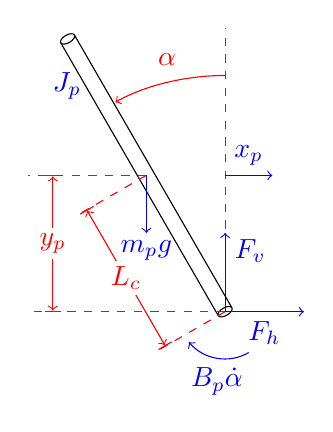
\begin{tikzpicture}
    \def\rodlength{40mm}
    \def\rodwidth{2mm}
    \begin{scope}[rotate=30]
        \draw (-0.5*\rodwidth, 0) -- (-0.5*\rodwidth, \rodlength);
        \draw (0.5*\rodwidth, 0) -- (0.5*\rodwidth, \rodlength);
        \draw ellipse [x radius=0.5*\rodwidth, y radius=0.25*\rodwidth];
        \draw[yshift=\rodlength] ellipse [x radius=0.5*\rodwidth, y radius=0.25*\rodwidth];
        \lineann{20mm}{90}{90}{1}{$L_c$}
    \end{scope}
    \lineann{20mm}{120}{90}{2.5}{$y_p$}
    \begin{scope}[rotate=90]
        \angann[3]{30}{$\alpha$}
    \end{scope}
    \draw[->, blue] (0, 17.3mm) -- node[above] {$x_p$} (6mm, 17.3mm);
    \draw[->, blue] (-10mm, 17.3mm) -- node[pos=1.3] {$m_p g$} (-10mm, 10mm);
    \draw[->, blue] (0, 0) -- node[above right] {$F_v$} (0, 10mm);
    \draw[->, blue] (0, 0) -- node[below] {$F_h$} (10mm, 0);
    \draw [->, blue] (-60:6mm) arc (-60:-140:6mm) node[midway, below] {$B_p \dot{\alpha}$};
    \node[blue] at (125:35mm) {$J_p$};
\end{tikzpicture}
